% Created 2022-01-26 Wed 15:35
% Intended LaTeX compiler: xelatex
\documentclass[11pt,twoside,landscape]{article}
\usepackage{graphicx}
\usepackage{longtable}
\usepackage{wrapfig}
\usepackage{rotating}
\usepackage[normalem]{ulem}
\usepackage{amsmath}
\usepackage{amssymb}
\usepackage{capt-of}
\usepackage{hyperref}
\usepackage[newfloat]{minted}
\usepackage{color}
\usepackage{listings}
\usepackage[top=2cm,bottom=2cm,right=2cm,left=2cm,landscape]{geometry}
\usepackage{multicol}
\usepackage{enumitem}
\usepackage{fancyhdr}
\setlist{noitemsep}
\setlength{\parindent}{0pt}
\setlength{\columnseprule}{0.2pt}
\definecolor{mygreen}{rgb}{0,0.6,0}
\definecolor{mygray}{rgb}{0.5,0.5,0.5}
\definecolor{mymauve}{rgb}{0.58,0,0.82}
\lstset{ backgroundcolor=\color{white}, basicstyle=\footnotesize, breaklines=true, captionpos=b, commentstyle=\color{mygreen}, escapeinside={\%*}{*)},keywordstyle=\color{blue}, stringstyle=\color{mymauve},}
\author{Olivier Lischer}
\date{\today}
\title{MsTe Summary}
\hypersetup{
 pdfauthor={Olivier Lischer},
 pdftitle={MsTe Summary},
 pdfkeywords={},
 pdfsubject={},
 pdfcreator={Emacs 27.2 (Org mode 9.5.2)}, 
 pdflang={English}}
\begin{document}

\pagestyle{fancy}
\fancyhf{}
\fancyhead[R]{MsTe-HS21}
\fancyhead[L]{Exam Summary}
\fancyfoot[CE,CO]{\leftmark}
\fancyfoot[R]{\thepage}
\fancyfoot[L]{Olivier Lischer}
\begin{multicols}{3}

\section{.NET}
\label{sec:org8e646cc}
\textbf{.NET}

\begin{itemize}
\item .NET Framework: only for Windows, no new Updates (except security patches)
\item .NET Core: new runtime, crossplatform
\item .NET: successor of .NET Core. This should be used today
\end{itemize}

\begin{figure}[htbp]
\centering
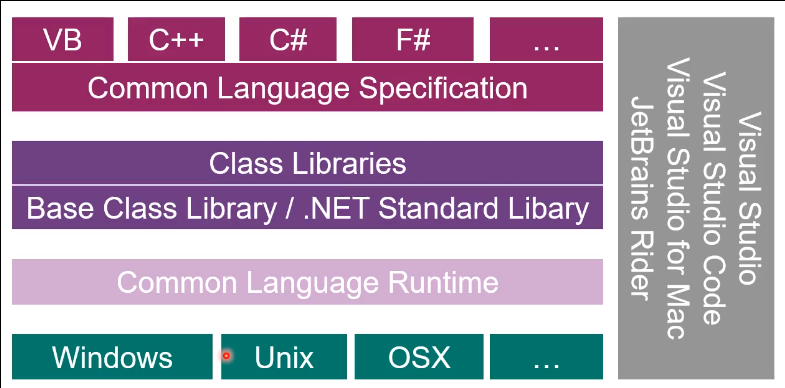
\includegraphics[width=.9\linewidth]{static/img/mste/dot_net_architektur.png}
\caption{\label{fig:orge2950db}.NET arcitecutre}
\end{figure}

\textbf{.NET Standard}

The .NET Stadard is used to establish a compatibility between different implementation.
The standard defines which functions, classes, etc. a implementation has to provided to be conform. 

\textbf{Common Language Runtime (CLR)}

The Common Language Runtime (CLR) has:
\begin{itemize}
\item a JIT Compiler which compiles the \href{../../../roam/20211003114528-microsoft_intermediate_language.org}{Microsoft Intermediate Language} to native code
\item Garbage Collection
\item inter language debugging
\item thread management
\end{itemize}


\begin{figure}[htbp]
\centering
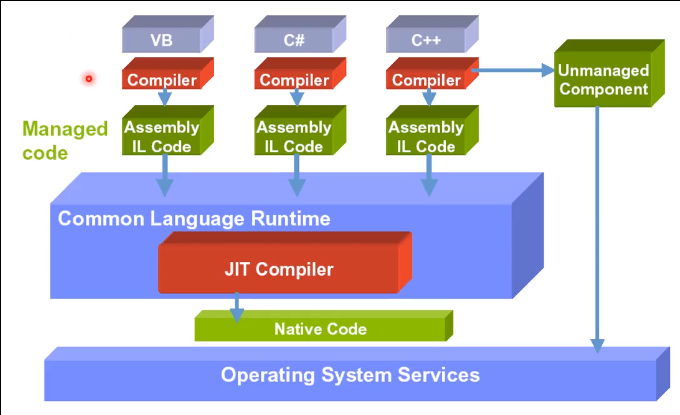
\includegraphics[width=.9\linewidth]{static/img/mste/clr_architektur.png}
\caption{\label{fig:org7cc7e5c}CLR Architecut}
\end{figure}

\textbf{Common Type System}

Common Type System (CTS) is the standard in \href{../../../roam/20211003114703-net.org}{.NET} how a type definitions and specific values are stored in memory.
All types in .NET inherit from \texttt{System.Object}. Also types like int, long and float inherit from \texttt{System.Object}. In CTS exists two different kind of types: Reference types (\texttt{class} keyword) and Value types (\texttt{struct} keyword). Value types are stored on the stack and are automatically boxed if it is used with something like a list, which stores its  element on the heap. 

\begin{table}[htbp]
\label{tab:orge6765b4}
\centering
\begin{tabular}{lll}
 & Reference (Class) & Value (Struct)\\
\hline
Memory Location & heap & stack\\
Variable contains & reference & value\\
Null value & possible & never\\
Default value & null & 0, false, '$\backslash$0'\\
Assignment / Call & copy reference & copy value\\
derivation possible & yes & no (sealed)\\
\end{tabular}
\end{table}

Each type has always a reference to the type description 

\begin{figure}[htbp]
\centering
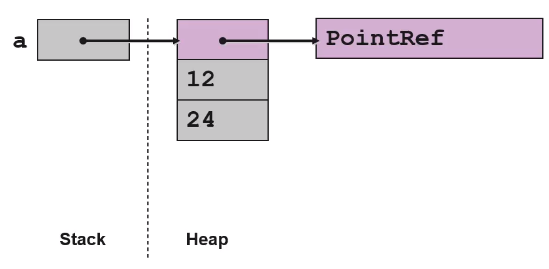
\includegraphics[width=.9\linewidth]{static/img/mste/ref_type_stack_heap.png}
\caption{\label{fig:org0fb3e9f}Example Memory Layout Reference}
\end{figure}

\textbf{.NET Assembly}

After the compilation you receive an Assembly.
This could be an *.exe or *.dll in Windows.
This Assembly is dynamically loadable and contains meta data.
It something like the JAR file in \href{../../../roam/20201116150053-java.org}{Java}.

\textbf{What contains a .NET Assembly?}

The Assembly contains:
\begin{itemize}
\item Manifest (references to other assemblies, metadata, version, author, \ldots{})
\item Module (types)
\item Resources  (images, translations files, \ldots{})
\end{itemize}


Module metadata:
\begin{itemize}
\item public, private, \ldots{}
\item describes all aspect of the code except programming logic
\item used to guarantee type safety
\item is normally used in IDEs to provide auto complition
\end{itemize}


\textbf{Microsoft Intermediate Language (MSIL)}

MSIL is similar to assembler but is platform independent.
The MSIL is the same for all \href{../../../roam/20211003114703-net.org}{.NET} languages.
The benefits of the MSIL are:
\begin{itemize}
\item portability
\item typesafety
\end{itemize}

The drawback is that the normal compiled project is not as efficient as native code.
But you can compile a \href{../../../roam/20211003114703-net.org}{.NET} project direct in native code.

\textbf{MSIL in Action}

\begin{itemize}
\item Design Time (platform independent, development, MSIL)
\item Run Time (platform dependent, JIT)
\end{itemize}

JIT Compilation:
compiled method calls an IL function.
The runtime detects that this function is not compiled yet and calls the JIT compiler.
The JIT compiler translate the IL code in native code and replace the IL code with native code in the memory.

\textbf{.NET reference types}

In \href{../../../roam/20211003114703-net.org}{.NET} exists 4 different kinds of references:
\begin{itemize}
\item precompiled assemblies (not possible to debug), \texttt{<Reference>..</Reference>}
\item \href{../../../roam/20211003140935-nuget_package.org}{NuGet Package} (external dependency, not possible to debug), \texttt{<PackageReference>...</PackageReference>}
\item Visual Studio Project (in same solution), \texttt{<ProjectReference>...</ProjectReference>}
\item SDK (required, default classes)
\end{itemize}


\textbf{C\# Project Files}

The \href{../../../roam/20211003114703-net.org}{.NET} project are store in a XML file.
In a \href{../../../roam/20211003114158-c.org}{C\#} project the file is called *.csproj.
The most important part in the file are:
\begin{itemize}
\item PropertyGroup: Settings
\item ItemGroup: item which should be compiled
\item TargetGroup: a sequence of step to execute
\end{itemize}


\section{C\#}
\label{sec:org1753f05}

\begin{figure}[htbp]
\centering
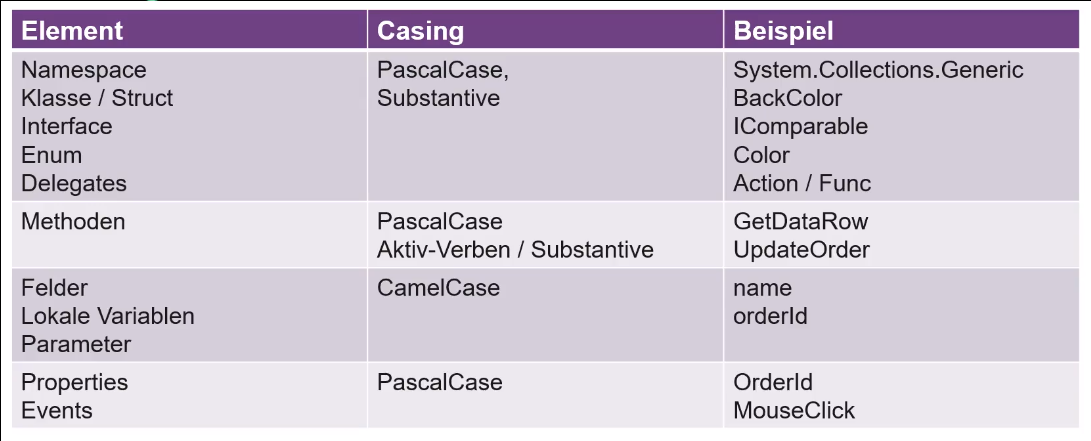
\includegraphics[width=.9\linewidth]{static/img/mste/naming_guidelines.png}
\caption{\label{fig:org497525f}Naming Guidelines}
\end{figure}

\begin{figure}[htbp]
\centering
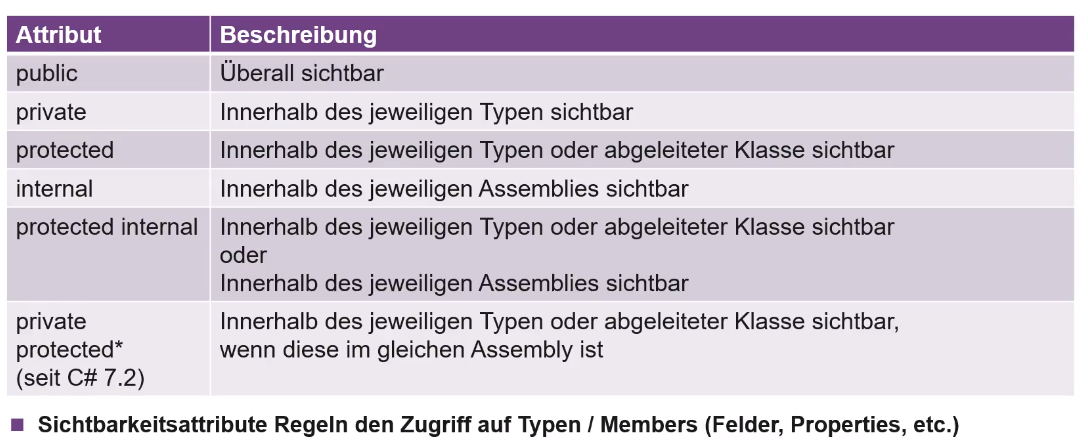
\includegraphics[width=.9\linewidth]{static/img/mste/sichtbarkeitsattribute.png}
\caption{\label{fig:org691e7d8}Visibility}
\end{figure}


\textbf{Namespaces in C\#}

Namespaces are similar to the packages in \href{../../../roam/20201116150053-java.org}{Java}.
But in \href{../../../roam/20211003114158-c.org}{C\#} the file systems does not have correspond the the namespace.
But it is best practice to have the same hierarchy.
A namespace can be renamed during the import: \texttt{using F = System.Windows.Forms}

\textbf{Main Method in C\#}

The main method in \href{../../../roam/20211003114158-c.org}{C\#} can exits mulitple times.
If this is the case the corret starting method has to written in the *.csproj file:

\lstset{language=XML,label= ,caption= ,captionpos=b,numbers=none}
\begin{lstlisting}
<StartupObject>CSharpGrundlagen_Main01.Program1</StartupObject>
\end{lstlisting}

\begin{figure}[htbp]
\centering
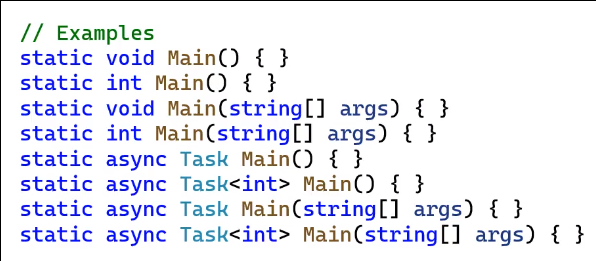
\includegraphics[width=.9\linewidth]{static/img/mste/main_methods_example.png}
\caption{\label{fig:orgb09b27a}Main Method Examples}
\end{figure}

Arguments can be access with:
\lstset{language=csharp,label= ,caption= ,captionpos=b,numbers=none}
\begin{lstlisting}
string[] args;
System.Environment.GetCommandLineArgs();
System.CommandLine; /*NuGet*/
\end{lstlisting}


The main method is not required.
If you leave out the main method (only allowed once) the following schema is required:
\begin{itemize}
\item usings
\item the code which is normaly in main
\item functions / enums / classes / structs \ldots{}
\end{itemize}


The argument array is then always called args.

\lstset{language=csharp,label= ,caption= ,captionpos=b,numbers=none}
\begin{lstlisting}
using System;

Volume vLow = Volume.Low;
PrintVolume(vLow);

static void PrintVolume(Volume volume) { /* */ }
public enum Volume { /* */ }
\end{lstlisting}

\textbf{Enums in C\#}

Enums in \href{../../../roam/20211003114158-c.org}{C\#} are only a list with predefined constants (default Int32).
Normally the first value is a 0 and the incremented.
It is possible to define the int value explicitly (\texttt{enum Days \{Sunday = 10, ... \}}.
After that the value is incremented again.
It is possible that the enum has for different options the same int value.
This could happens when you set one option explicit higher and one option explicit lower.
In this case it is not recommended to convert the int in an enum (it will always take only the first option).

To save memory you can adjust the used type \texttt{enum Days : byte \{ Sunday, Monday ... \};}.
This is \emph{not in inheritance}. Just a hint for the compiler.

\textbf{String to Enum}

Often you want to convert a String into an Enum (\href{../../../roam/20211006113326-enums_in_c.org}{Enums in C\#}).
For this operation you have to options:
\begin{itemize}
\item The Option 1 should not be used anymore, because it can throw exceptions
\item Option 2 and 3 are identical except that Option 3 has same syntactical sugar.
\end{itemize}

\lstset{language=csharp,label= ,caption= ,captionpos=b,numbers=none}
\begin{lstlisting}
// Option 1
Days day1 = (Days)Enum.Parse(typeof(Days), "Monday");

// Option 2
Days day2;
bool success2 = Enum.TryParse("Monday", out day2);

// Option 3
bool success3 = Enum.TryParse("Monday", out Days day3); // C# 7.0
\end{lstlisting}

\textbf{Print all Options of an Enum}

Sometimes you want to iterate over all Values of a enum (\href{../../../roam/20211006113326-enums_in_c.org}{Enums in C\#}).

\lstset{language=csharp,label= ,caption= ,captionpos=b,numbers=none}
\begin{lstlisting}
foreach (string day in Enum.GetNames(typeof(Days)))
{
    Console.WriteLine(day);
}
\end{lstlisting}

\textbf{String in C\#}

The type string is a reference type (class) but behaves like a Value type and are reused internally.
Only \texttt{string.Copy()} creates a real new copy.
Strings are immutable and value comparison with \texttt{=} / \texttt{!=} and \texttt{Equals} are possible (not like in \href{../../../roam/20201116150053-java.org}{Java}).
For escaping two methods exist:
\begin{itemize}
\item escaping with a backslash ($\backslash$): \texttt{"C:\textbackslash{}\textbackslash{}"}
\item or with a at @: \texttt{@"C:\textbackslash{}"}
\end{itemize}


Strings should not be created with \texttt{string.Format()} or with the \texttt{+} operator.
The better way is string interpolation: \texttt{string s3 = \$"\{DateTime.Now\}: \{"Hello"\}";}

\textbf{Arrays in C\#}

In \href{../../../roam/20211003114158-c.org}{C\#} the array is a reference type is therefore stored on the heap.
It exists three different kind of arrays:
\begin{itemize}
\item \href{../../../roam/20211008083138-single_dimensional_arrays_in_c.org}{Single Dimensional Arrays in C\#}
\item \href{../../../roam/20211008083241-multidimension_array_in_c.org}{Multidimension Array in C\#}
\item \href{../../../roam/20211008083300-jagged_arrays_in_c.org}{Jagged Arrays in C\#}
\end{itemize}


If the array stores reference types then only the reference is stored in the array. If the array should store value types then these elements are automatically boxed (moved to the heap) and stored as a whole in the array.

\begin{figure}[htbp]
\centering
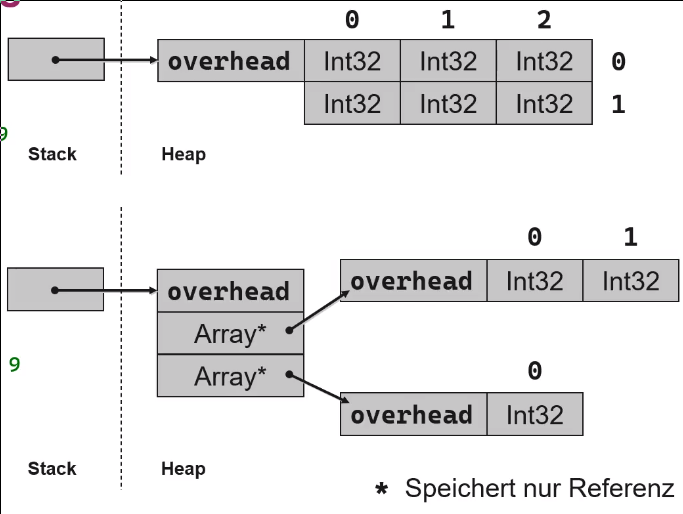
\includegraphics[width=.9\linewidth]{static/img/mste/array_memory_layout.png}
\caption{\label{fig:org4248a2f}Array Memory Layout}
\end{figure}

\textbf{Single Dimensional Array}

An plan old array. Nothing special.
\lstset{language=csharp,label= ,caption= ,captionpos=b,numbers=none}
\begin{lstlisting}
int[] array1 = new int[5];
int[] array2 = new int[] { 1, 4, 6};
int[] array3 = int[] {1,5,7};
int[] array4 = {1,3,5,5};
object[] array5 = new object[5];
\end{lstlisting}

\textbf{Multidimensional Array}

Multidimensional Arrays are also called Block Matrices because they look like a rectangle.

\lstset{language=csharp,label= ,caption= ,captionpos=b,numbers=none}
\begin{lstlisting}
int[,] multiDim1 = new int[2,3];
int[,] multiDim2 = new { {1,2,3}, {4,5,6}};

int[,] array = new int[3,2];
int length = array.Length; // 6
int length0 = array.GetLength(0); // 3
int length1 = array.GetLength(1); // 2
\end{lstlisting}


The benefits over \href{../../../roam/20211008083300-jagged_arrays_in_c.org}{Jagged Arrays in C\#} they are:
\begin{itemize}
\item more memory efficient
\item faster allocation
\item faster \href{../../../roam/20211008083744-garbage_collection.org}{Garbage Collection}
\end{itemize}


But the access to the elements are slower than in a \href{../../../roam/20211008083300-jagged_arrays_in_c.org}{Jagged Arrays in C\#}.
This is because the Boundary Check is in a \href{../../../roam/20211008083138-single_dimensional_arrays_in_c.org}{One Dimensional Array} is optimized.
This does not apply for Block Matrices. 

\textbf{Jagged Arrays}

Jagged Arrays are Arrays of Arrays.
From the first array, each index points to an indepentend Array.
They are called jagged (de: zerklüftet) because each array from the second array can have diffrent sizes.

\lstset{language=csharp,label= ,caption= ,captionpos=b,numbers=none}
\begin{lstlisting}
int[][] jaggedArray = new int[6][];
jaggedArray[0] = new int[] {1,2,3,4};

int[][] array1 new int[2][];
array1[0] = new int[3];
array1[1] = new int[1];
int length = array1.Length; // 2
int length0 = array1[0].Length; // 3
int length1 = array1[1].Length // 1
\end{lstlisting}

The access to the elements is in Jagged Arrays faster than in \href{../../../roam/20211008083241-multidimension_array_in_c.org}{Block Matrices} because the Boundary Check is for \href{../../../roam/20211008083138-single_dimensional_arrays_in_c.org}{One Dimensional Array} optimized.

\textbf{Structs in C\#}

In \href{../../../roam/20211003114158-c.org}{C\#} \texttt{struct} are value types and therefore live on the stack.
Derivation of a struct is not possible but a struct can implement interfaces.
Different as by classes you can not initialize the values directly:
\lstset{language=csharp,label= ,caption= ,captionpos=b,numbers=none}
\begin{lstlisting}
struct Point {
    int x = 0; // Compilerrror
    int y;

    Point(int x, int y) {
	this.x = x;
	this.y = y;
    }
}

\end{lstlisting}


Structs should only used in the following cases:
\begin{itemize}
\item to group primitives as one data type (like a Point)
\item the new type should be immutable
\item is not often boxed
\item short life span
\item or is embedded in other objects
\end{itemize}


\textbf{readonly fields}

In \href{../../../roam/20211003114158-c.org}{C\#} besides \texttt{const} there is also a \texttt{readonly}.
The value for a \texttt{readonly} fields does not have to be known at compile time.
The value can be calculated during deklaration or inside the constructor.

\textbf{nested types in}

The outer class has access to the public functions / fields / properties of the class.
But the inner class has access to everything of the outer class.
Foreign classes can access only on public functions / fields / properties and only if the class itself is public.

\textbf{Static Usings}

In \href{../../../roam/20211003114158-c.org}{C\#} you can import static classes / enums with static usings:
\lstset{language=csharp,label= ,caption= ,captionpos=b,numbers=none}
\begin{lstlisting}
using static System.Console;

WriteLine("Hello World");
\end{lstlisting}

If a naming clash occurs the normal overloading rules apply.
With the class name you can ensure the correct function call.

\textbf{Params}

In \href{../../../roam/20211003114158-c.org}{C\#} exists two kind of functions calls:
\begin{itemize}
\item call by value
\item call by reference
\end{itemize}


For call by reference exists two keywords with different purpose:
\begin{itemize}
\item \texttt{ref} (normal call be reference)
\item \texttt{out}
\end{itemize}


For overloading \texttt{ref} / \texttt{out} are distinguished feature.

\textbf{out Parameters}

A function which takes \texttt{out} parameters initialized this arguments during the function call.
This technique is used by the \texttt{TryParse} methods.
If you are not interested in one of the parameters then use the \texttt{\_} to discard the "return value".

\lstset{language=csharp,label= ,caption= ,captionpos=b,numbers=none}
\begin{lstlisting}
void Init(out int a, out int b) { a = 1; b = 2; }
void TestInit() { Init(out int a1, out _); }
\end{lstlisting}

\textbf{params array}

The params array allows the caller to add any number of arguments at the end:
\lstset{language=csharp,label= ,caption= ,captionpos=b,numbers=none}
\begin{lstlisting}
void DoSomething(string str, params string[] list) { /**/ }
DoSomething("{0} some string {1}", 2, 3); 
\end{lstlisting}

It has to be the last parameter in the function. During compilation time the parameters are transformed in an normal array. It is not possible to use the parms array with the \texttt{out} / \texttt{ref} keyword.

\textbf{Imporent}: the following two functions are the same for the compiler (no valid overloading):
\lstset{language=csharp,label= ,caption= ,captionpos=b,numbers=none}
\begin{lstlisting}
void DoSomething(string str, params string[] list) { /**/ }
void DoSomething(string str, string[] list) { /**/ }
\end{lstlisting}

\textbf{Optional Parameters}

In \href{../../../roam/20211003114158-c.org}{C\#} exist optional parameters.
This is realized that some parameters have a default value:
\lstset{language=csharp,label= ,caption= ,captionpos=b,numbers=none}
\begin{lstlisting}
void optionalParameters(int i, bool flag = true) { /**/ }
\end{lstlisting}

The default value has be calculated during compile time.
Leaving out an optional parameter is only possible at the end.
If you want to specify the last option then you have set all previous flags too.

\textbf{Important}: Default parameters are no distinguished feature for overloading.
The following are the same function for the compiler (compiler error):
\lstset{language=csharp,label= ,caption= ,captionpos=b,numbers=none}
\begin{lstlisting}
void optionalParameters(int i, bool flag = true) { /**/ }
void optionalParameters(int i, bool flag) { /**/ }
\end{lstlisting}

\textbf{Named Parameters}

The problem with \href{../../../roam/20211008100451-optional_parameters_in_c.org}{Optional Parameters in C\#} is that you have sometimes to specify every option even if you want only to change the default value of the last argument.
With named parameters this problem does not occur:
\lstset{language=csharp,label= ,caption= ,captionpos=b,numbers=none}
\begin{lstlisting}
void PrintOrderDetails(string productName, string sellerName, int orderNum) { /**/ }
PrintOrderDetails(orderNum: 31, productName: "Red Mug", sellerName: "Gift Shop");
\end{lstlisting}

\textbf{Properties}

Properties are compiler feature which implements the Getter and Setter methods.
In the Set part you can access the assigned value using the \texttt{value} keyword.

\lstset{language=csharp,label= ,caption= ,captionpos=b,numbers=none}
\begin{lstlisting}
public int LengthAuto { get; set; }
\end{lstlisting}

Auto implemented properties use compiler also a compiler feature.
To avoid naming conflicts the compiler creates a "unspeakable variable name".
This is a variable name which the compiler not accepted from the user.

You can even initialized auto implemented properties.
The set part does not even to be there.
\lstset{language=csharp,label= ,caption= ,captionpos=b,numbers=none}
\begin{lstlisting}
public string FirstName { get; set; } = "Jane"; 
\end{lstlisting}


Another compiler feature is that you can set the values over the Setters right after the creation using the default compiler:
\lstset{language=csharp,label= ,caption= ,captionpos=b,numbers=none}
\begin{lstlisting}
MyClass mc = new MyClass()
{
    Length = 1,
    Width = 2
};

// compiles to this
MyClass mc = new MyClass();
mc.Length = 1;
mc.Width = 2;
\end{lstlisting}

\textbf{Indexers}

Indexer are just a special case of \href{../../../roam/20211008103108-properties_in_c.org}{Properties in C\#}.
It is basically an overloading of the index operator (\texttt{[]}):
\lstset{language=csharp,label= ,caption= ,captionpos=b,numbers=none}
\begin{lstlisting}
MyClass mc = new MyClass();
mc[0] = "Hello";
string value1 = mc[0];

class MyClass
{
    private string[] arr = new string[10];
    // this zeigt an dass es ein indexer ist
    public string this[int index]
    {
	get { return arr[index]; }
	set { arr[index] = value; // value ist ein string in diesem fall }
    }

}
\end{lstlisting}

\textbf{Switch Expressions}

The switch expression in \href{../../../roam/20211003114158-c.org}{C\#} works like the switch expression in \href{../../../roam/20200904153952-rust.org}{Rust}.

\lstset{language=csharp,label= ,caption= ,captionpos=b,numbers=none}
\begin{lstlisting}
public static Orientation ToOrientation(Direction direction) => direction switch
{
    Direction.Up    => Orientation.North,
    Direction.Right => Orientation.East,
    Direction.Down  => Orientation.South,
    Direction.Left  => Orientation.West,
    _ => throw new ArgumentOutOfRangeException(nameof(direction), $"Not expected direction value: {direction}"),
};
\end{lstlisting}

\textbf{Default in C\#}

In \href{../../../roam/20211003114158-c.org}{C\#} for a \href{../../../roam/20211008085202-struct_in_c.org}{Struct in C\#} the default constructor is always available.
For a class when no constructor is implemented by the user or explicitly implemented.
In a \href{../../../roam/20211008085202-struct_in_c.org}{Struct in C\#} always all fields have to be initialized.

Using \texttt{default(T)} or \texttt{default} the memory location is filled with 0.
So the get the default value back.

\textbf{Static Constructors}

A static constructor is for structs and classes identically and has never parameters and no visibility.
The static constrocutr is used for initial work and is executed exactly once for the whole application during the first creation of an object of the class / struct.

\textbf{Operator Overloading}

The function has to be a \texttt{static} and needs the keyword \texttt{operator} with the operator afterwards:
\lstset{language=csharp,label= ,caption= ,captionpos=b,numbers=none}
\begin{lstlisting}
public static Point operator+(Point lhs, Point rhs) {
    return new Point(rhs.X + lhs.X, rhs.Y + lhs.Y);
}
\end{lstlisting}

The return type freely selectable.
But min. one parameter has to be from the same type of the class.

\textbf{Partial Class}

A class can be spitted in multiple files.
This requires the keyword \texttt{partial}.
This works with classes, structs and interfaces.
\lstset{language=csharp,label= ,caption= ,captionpos=b,numbers=none}
\begin{lstlisting}
// File1.cs
partial class MyClass
{
    public void Test1() {}
}

// File2.cs
partial class MyClass
{
    public void Test2() {}
}
\end{lstlisting}

Usage:
\begin{itemize}
\item Mostly used with generators:
\begin{itemize}
\item File 1: created by the generator
\item File 2: created by the developer
\end{itemize}
\item Split up a big file (bad code)
\begin{itemize}
\item good starting point for refactoring
\end{itemize}
\end{itemize}


If I define in one place partially this is valid for all other files too.

\textbf{Partial Method}

It is also possible to implement partial methods.
This is often used for user defined hooks in generated code.
For this the class / struct needs to be also partial and the function has to be private and has to return void.

\lstset{language=csharp,label= ,caption= ,captionpos=b,numbers=none}
\begin{lstlisting}
// Definition in file1.cs, e.g generated by an generator
partial void OnNameChanged();

// Implementation in file2.cs, implemented by an developer
partial void OnNameChanged() { /**/ }
\end{lstlisting}


\begin{figure}[htbp]
\centering
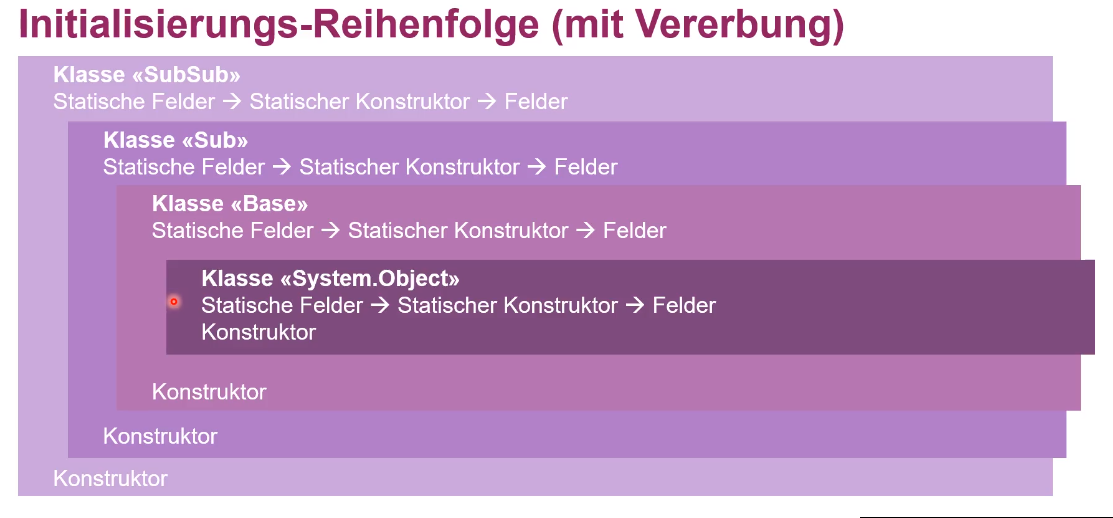
\includegraphics[width=.9\linewidth]{static/img/mste/initialisierungsreihenfolge.png}
\caption{\label{fig:org51b4c57}Initialisierungsreihenfolge}
\end{figure}

\textbf{Type Casting}

\texttt{null} could be also casted.
Except you want to cast it in a Value Type (\href{../../../roam/20211008085202-struct_in_c.org}{Struct in C\#}).
This would throw an \texttt{InvalidCastException}.
\lstset{language=csharp,label= ,caption= ,captionpos=b,numbers=none}
\begin{lstlisting}
SubSub a = new SubSub();
if (a is SubSub) {}
\end{lstlisting}

\texttt{obj as T} short for \texttt{obj is T ? (T)obj : (T)null}
\lstset{language=csharp,label= ,caption= ,captionpos=b,numbers=none}
\begin{lstlisting}
Base a = new Sub();
Sub b = a as Sub;

/* Same as following*/
Sub b = a is Sub ? (Sub)a : (Sub)null;
\end{lstlisting}

\lstset{language=csharp,label= ,caption={type check with implicit type cast},captionpos=b,numbers=none}
\begin{lstlisting}
Base a = new SubSub();
if (a is SubSub casted) {
    Console.WriteLine(casted);
}

/* same as following*/ 
SubSub casted = default;
if (a is SubSub) {
    casted = (SubSub) a;
}
\end{lstlisting}

\textbf{Override Functions}

So that you can override a function it has to be marked as \texttt{virtual} in the base class.
In the child class you can override it with the keyword \texttt{override}.
The keyword \texttt{virtual} is not possible when:
\begin{itemize}
\item function is static
\item function is \texttt{abstract} (implied virtual)
\item private (not even possible to override)
\item override (implied virtual from base class)
\end{itemize}


\textbf{Dynamic Binding in C\#}

Rule Set in pseudo code:
\lstset{language=csharp,label= ,caption= ,captionpos=b,numbers=none}
\begin{lstlisting}
var st = static type of obj;
var dt = dynamic type of obj;
var m = Method "M" of st; // Standard-Methode, existiert zwingend (evtl. vererbt)!
var typelist = all types between st (exclusive) and dt (inclusive);

foreach (var t in typelist)
{
    // Schlüsselwort "override"
    if (t has an override method "M")
	m = Method "M" of t;
    // Schlüsselwort "new"
    // Oder ohne Angabe
    else if (t has a non-override method "M")
	break;
}
call m;
\end{lstlisting}

\textbf{Interrupt dynamic binding}

If the keyword \texttt{override} is missing the original functions are hidden therefore the dynamic binding is interrupted.
If you want this you should add the \texttt{new} keyword: \texttt{public new void I() \{\}}.
This tells the compiler that you really want this and it is not a mistake.

\textbf{seald keyword}

With the keyword \texttt{sealed} you prevent that something inherits from this.
\texttt{sealed} can be used with classes, properties, indexers and events.

\texttt{sealed} can improve the performance because the dynamic binding algorithm is not executed.

sealed members are not very common and are only possible with the keyword \texttt{override}:
\begin{itemize}
\item \texttt{public override sealed void Add()}
\end{itemize}


But you can hide the sealed function and create a new hierarchy with the \texttt{new} keyword:
\begin{itemize}
\item \texttt{public new virtual void Add()}
\end{itemize}


\textbf{Interfaces in C\#}

Because \href{../../../roam/20211003114158-c.org}{C\#} does not allow multiple inheritance the Interfaces are created.
A class can implemented multiple interfaces at the same time.
All function defined in the interface must be implemented by the class or by a base class.
Implementation of Interface members must be \texttt{public} and must not be \texttt{static}.
Interfaces can inherit from other Interfaces

\textbf{Naming Clashes using Interfaces}

If your class implements two interfaces with the same name and same signature you have 3 possible solutions:
\begin{enumerate}
\item implement the method regularly.
The implementation counts for both interfaces
\begin{itemize}
\item do this if the logic for both interfaces are the same
\end{itemize}
\item implement the methods explicit
\begin{itemize}
\item do this if the logic for both interfaces are different
\item \texttt{void ISequence.Add(object x) \{ /* do something */ \}}
\item \texttt{void IShoppingCart.Add(object x) \{ /* do something */ \}}
\end{itemize}
\item implement one regularly and one explicit
\begin{itemize}
\item this is useful if the regularly one should be the default
\end{itemize}
\end{enumerate}

\lstset{language=csharp,label= ,caption={Prevent naming clash with option 2},captionpos=b,numbers=none}
\begin{lstlisting}
class ShoppingCart : ISequence, IShoppingCart {
    void ISequence.Add(object x) {}
    void IShoppingCart.Add(object x) {}
}

ISequence sc1 = new ShoppingCart();
sc1.Add("Hello");

IShoppingCart sc2 = new ShoppingCart();
sc2.Add("Hello");
\end{lstlisting}

\lstset{language=csharp,label= ,caption={Prevent naming clash with option 3},captionpos=b,numbers=none}
\begin{lstlisting}
class ShoppingCart : ISequence, IShoppingCart {
    void Add(object x) {} // will be the default
    void IShoppingCart.Add(object x) {}
}
\end{lstlisting}


\section{End}
\label{sec:org5d2da38}
\end{multicols}
\end{document}